 \documentclass[oneside,a4paper,14pt]{extarticle}
\usepackage[T1,T2A,TU]{fontenc}
\usepackage[a4paper,letterpaper,top=20mm,bottom=20mm,left=20mm,right=10mm]{geometry}
\usepackage[russian]{babel}
\usepackage{textcomp}
\usepackage{indentfirst}
\usepackage{graphicx}
\usepackage{mwe}
\usepackage{wrapfig}
\usepackage{caption}
\usepackage{amsmath}
\usepackage{amsfonts}
\usepackage{amsthm}
\usepackage{amssymb}
\usepackage[all]{xy}
\usepackage[breaklinks]{hyperref}
\usepackage{titlesec}
\usepackage{verbatim, fancyvrb}

\titleformat{\section} % Настройка формата заголовков секций
{\normalsize\bfseries} % Устанавливает размер шрифта на нормальный и делает его жирным
{\thesection} % Указывает, что номер секции будет отображаться перед заголовком
{1em} % Устанавливает расстояние между номером секции и заголовком в 1em
{} % Дополнительные параметры.

\titleformat{\subsection} % Настройка формата заголовков подсекций
{\normalsize\bfseries} % Устанавливает размер шрифта на нормальный и делает его жирным
{\thesubsection} % Указывает, что номер подсекции будет отображаться перед заголовком
{1em} % Устанавливает расстояние между номером подсекции и заголовком в 1em
{} % Дополнительные параметры.

\titleformat{\subsubsection} % Настройка формата заголовков подподсекций
{\normalsize\bfseries} % Устанавливает размер шрифта на нормальный и делает его жирным
{\thesubsection} % Указывает, что номер подподсекции будет отображаться перед заголовком
{1em} % Устанавливает расстояние между номером подподсекции и заголовком в 1em
{} % Дополнительные параметры.

\renewcommand\baselinestretch{1.45}\normalsize %межстр интервал
\setlength{\parindent}{1.25cm} %длина отступа нового абзаца

\begin{document}
\newpage
\thispagestyle{empty}
\begin{center}
	МИНИСТЕРСТВО НАУКИ И ВЫСШЕГО ОБРАЗОВАНИЯ\\
	РОССИЙСКОЙ ФЕДЕРАЦИИ
	ФЕДЕРАЛЬНОЕ ГОСУДАРСТВЕННОЕ БЮДЖЕТНОЕ\\
	ОБРАЗОВАТЕЛЬНОЕ
	УЧРЕЖДЕНИЕ ВЫСШЕГО ОБРАЗОВАНИЯ\\
	«ВЯТСКИЙ ГОСУДАРСТВЕННЫЙ УНИВЕРСИТЕТ»\\
	Институт математики и информационных систем\\
	Факультет автоматики и вычислительной техники\\
	Кафедра электронных вычислительных машин
\end{center}
\vspace{20mm}

\begin{center}
	Отчёт по лабораторной работе №4\\
	по дисциплине\\
	<<Информатика>>\\
	<<Форматы представления числовой информации. Представление целых чисел.>>\\
\end{center}
\vspace{40mm}
\noindent
  \begin{tabular}{ll}
    Разработал студент гр. ИВТб-1301-05-00 & \rule[-1mm]{30mm}{0.10mm}\,/Черкасов А. А./\\
    & \hspace{8mm}\footnotesize(подпись)\\
     
    Проверил доцент кафедры ЭВМ & \rule[-1mm]{30mm}{0.10mm}\,/Коржавина А.С./\\
    & \hspace{8mm}\footnotesize(подпись)\\
  \end{tabular}

\vfill
\begin{center}
	Киров\\
	2024
\end{center}

\newpage\thispagestyle{plain}
\section*{Цель работы}
Цель работы: Закрепить на практике знания форматах представления числовой информации.
Написать программы, решающие описанные ниже задачи.

\section*{Задания}
\begin{enumerate}
    \item \textbf{Представление беззнакового числа в $n$-разрядной сетке.}\\
          На вход подаётся целое число в десятичной системе и разрядность сетки. Если число отрицательное или превышает допустимое значение для данной разрядности, выводится ошибка.\\
          \textbf{Формат ввода.} \\
          В одной строке через пробел вводятся число и разрядность сетки.\\
          \textbf{Формат вывода.} \\
          Вывести строку, представляющую число в $n$-разрядной сетке или сообщение об ошибке.\\
          $$
          \begin{tabular}{ll}
          \textbf{Ввод} & \textbf{Вывод} \\
          \hline
          1 8           & 00000001       \\
		  \hline
          255 8         & 11111111       \\
		  \hline
          256 8         & ошибка         \\
          \hline
          \end{tabular}
          $$

    \item \textbf{Представление числа в прямом коде.}\\
          На вход подаётся целое число и разрядность сетки. Если число выходит за пределы представления в данной разрядности, выводится ошибка. Прямой код формируется как для положительных, так и отрицательных чисел.\\
          \textbf{Формат ввода.} \\
          В одной строке через пробел вводятся число и разрядность сетки.\\
          \textbf{Формат вывода.} \\
          Вывести строку, представляющую число в прямом коде или сообщение об ошибке.\\
          $$
          \begin{tabular}{ll}
          \textbf{Ввод} & \textbf{Вывод} \\
          \hline
          -1 8          & 10000001       \\
		  \hline
          25 8          & 00011001       \\
		  \hline
          -128 8        & ошибка         \\
          \hline
          \end{tabular}
          $$

    \item \textbf{Представление числа в дополнительном коде.}\\
          На вход подаётся целое число и разрядность сетки. Если число выходит за пределы представления, выводится ошибка.\\
          \textbf{Формат ввода.} \\
          В одной строке через пробел вводятся число и разрядность сетки.\\
          \textbf{Формат вывода.} \\
          Вывести строку, представляющую число в дополнительном коде или сообщение об ошибке.\\
          $$
          \begin{tabular}{ll}
          \textbf{Ввод} & \textbf{Вывод} \\
          \hline
          -1 8          & 11111111       \\
		  \hline
          25 8          & 00011001       \\
		  \hline
          225 8         & ошибка         \\
          \hline
          \end{tabular}
          $$

    \item \textbf{Представление числа в обратном коде.}\\
          На вход подаётся целое число и разрядность сетки. Если число выходит за пределы представления, выводится ошибка.\\
          \textbf{Формат ввода.} \\
          В одной строке через пробел вводятся число и разрядность сетки.\\
          \textbf{Формат вывода.} \\
          Вывести строку, представляющую число в обратном коде или сообщение об ошибке.\\
          $$
          \begin{tabular}{ll}
          \textbf{Ввод} & \textbf{Вывод} \\
          \hline
          -1 8          & 11111110       \\
		  \hline
          25 8          & 00011001       \\
		  \hline
          -168 8        & ошибка         \\
          \hline
          \end{tabular}
          $$

    \item \textbf{Расстояние по Хэммингу двух дополнительных кодов.}\\
          На вход подаются два числа и разрядность сетки. Преобразуются числа в дополнительные коды и вычисляется количество отличающихся позиций.\\
          \textbf{Формат ввода.} \\
          В одной строке вводятся два числа и разрядность сетки.\\
          \textbf{Формат вывода.} \\
          Вывести расстояние по Хэммингу или сообщение об ошибке.\\
          $$
          \begin{tabular}{ll}
          \textbf{Ввод} & \textbf{Вывод} \\
          \hline
          -1 25 8       & 7              \\
		  \hline
          -1 225 8      & ошибка         \\
          \hline
          \end{tabular}
          $$
\end{enumerate}
\newpage

\section*{Решение}
\noindent Схема алгоритма представлена на Рисунках 1.1 и 1.2. \\
\noindent Код программы приведён в Приложении A1.\\
\begin{figure}[h!]
    \centering
    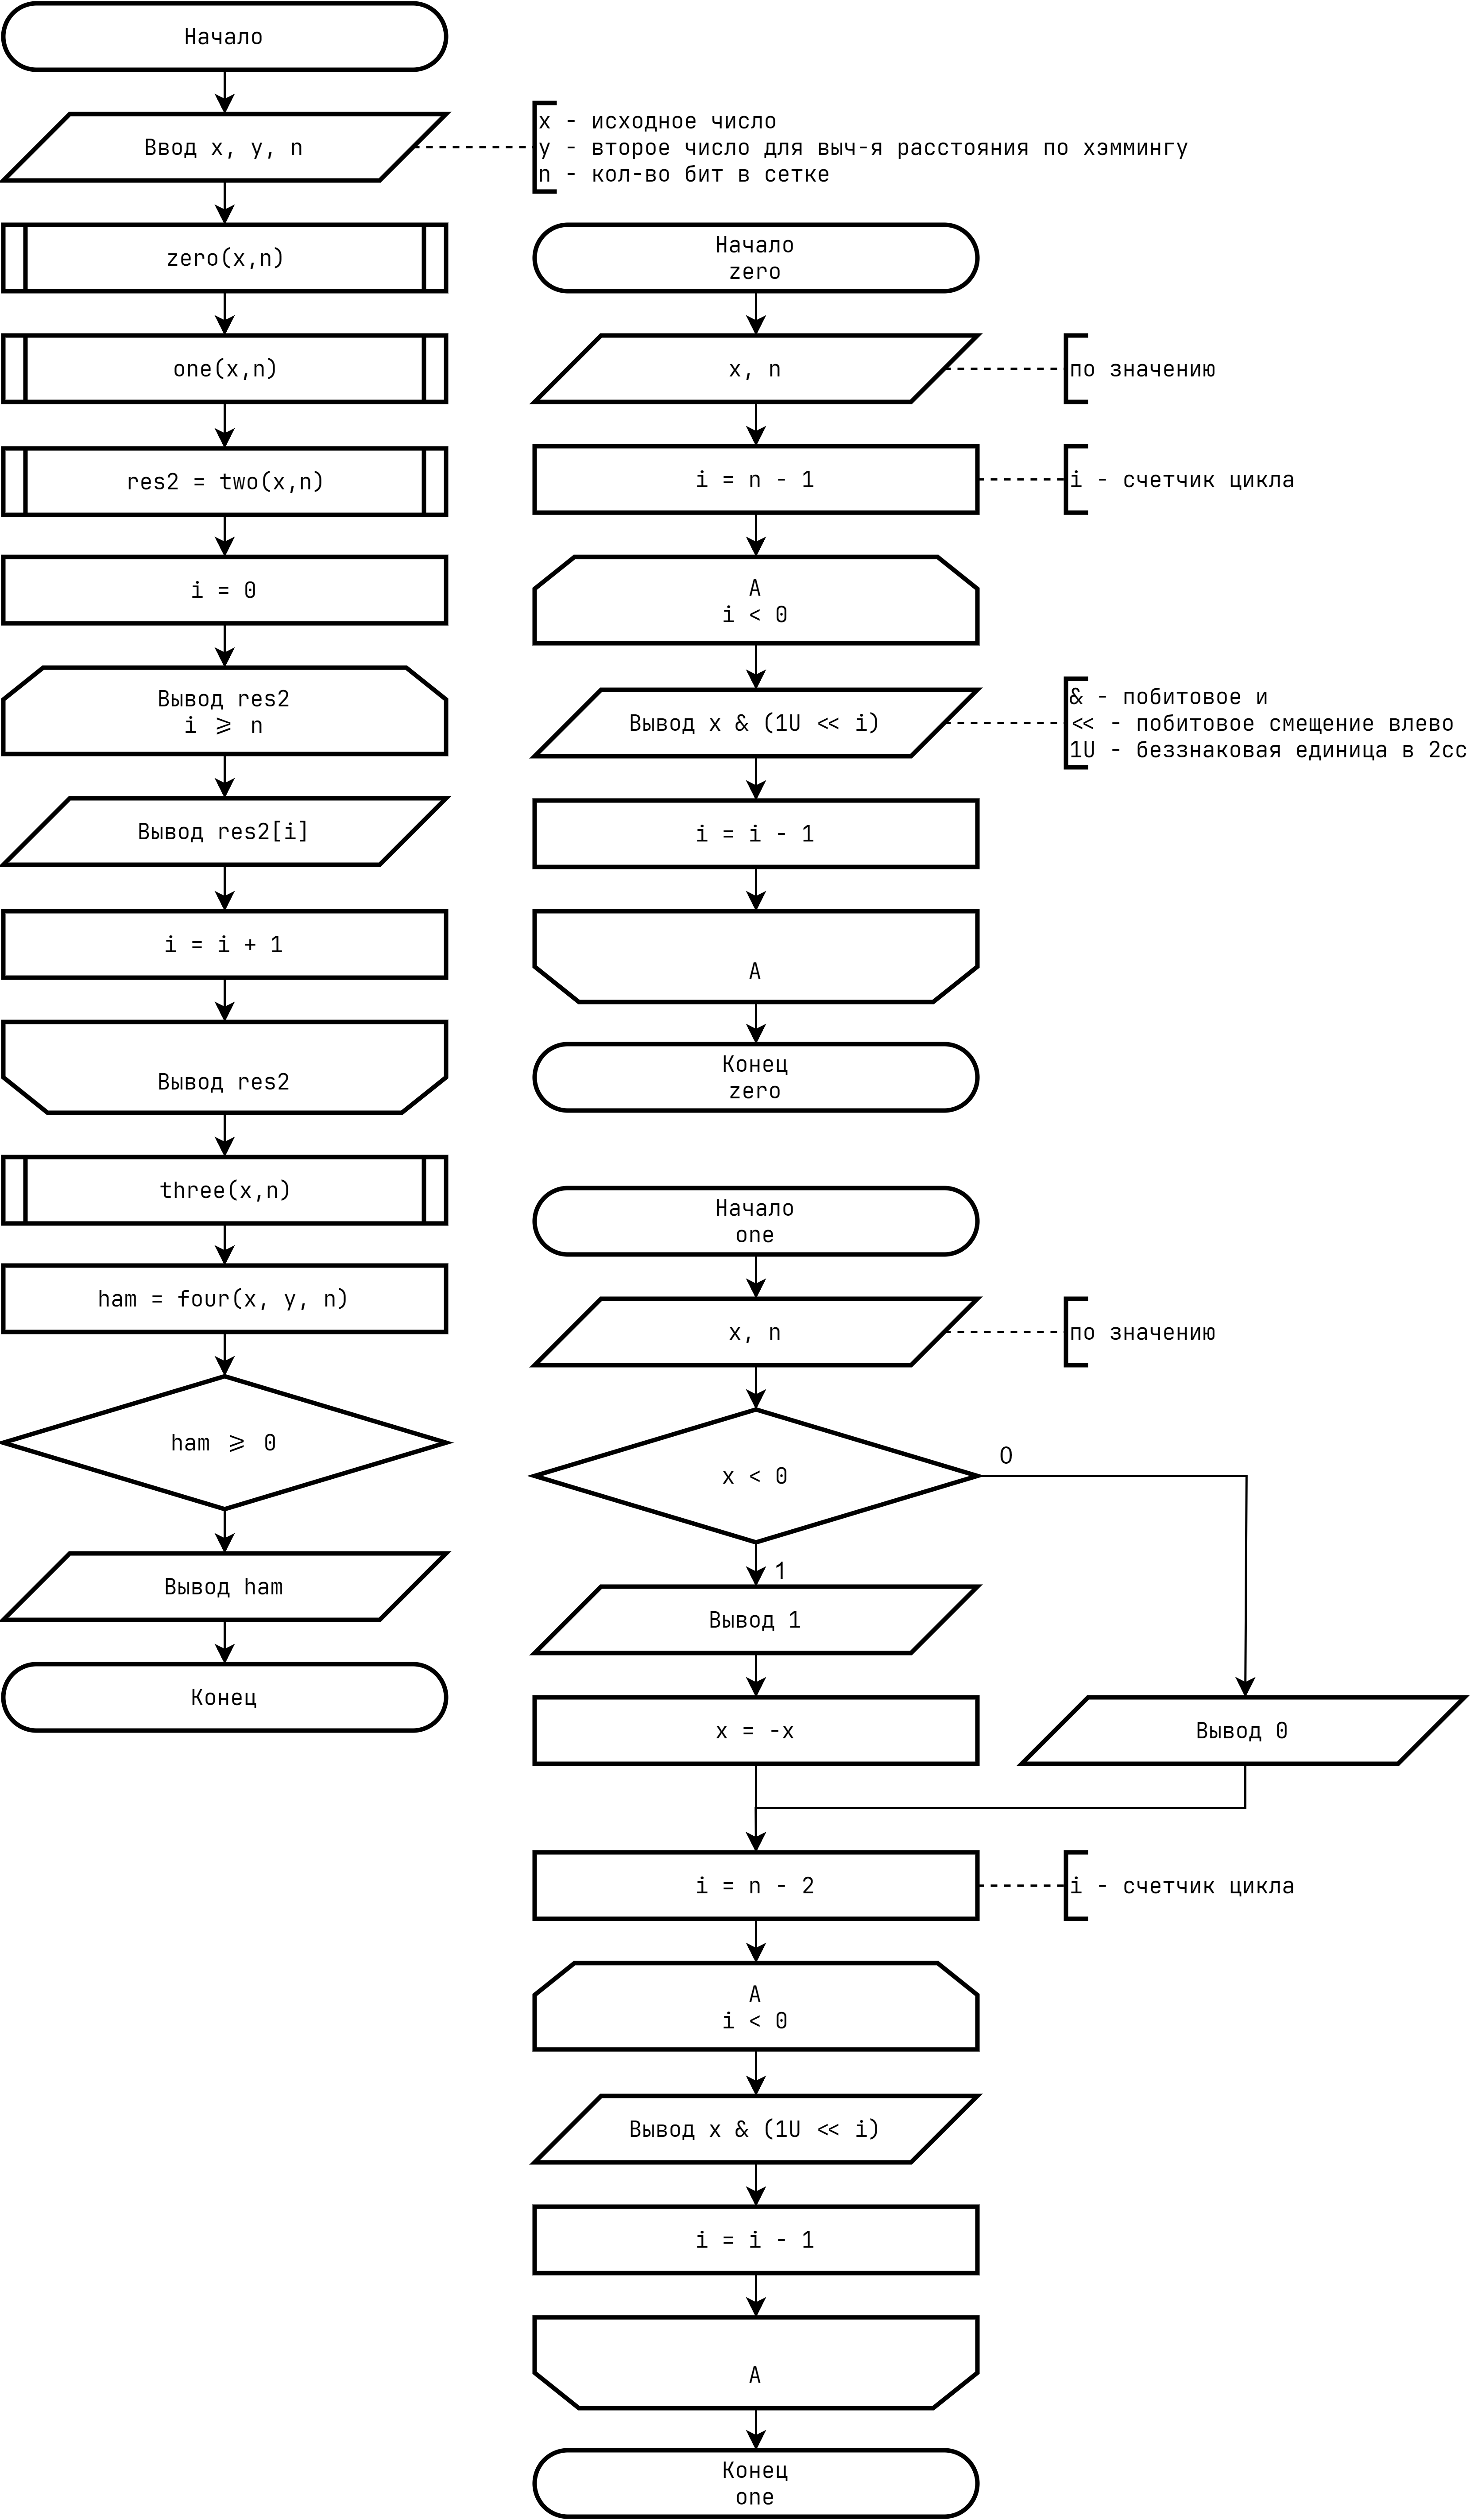
\includegraphics[height=0.75\textheight]{pics/flowchart_p1.png}
    \caption*{Рисунок 1.1 - Схема алгоритма программы.}
\end{figure}

\begin{figure}[h!]
    \centering
    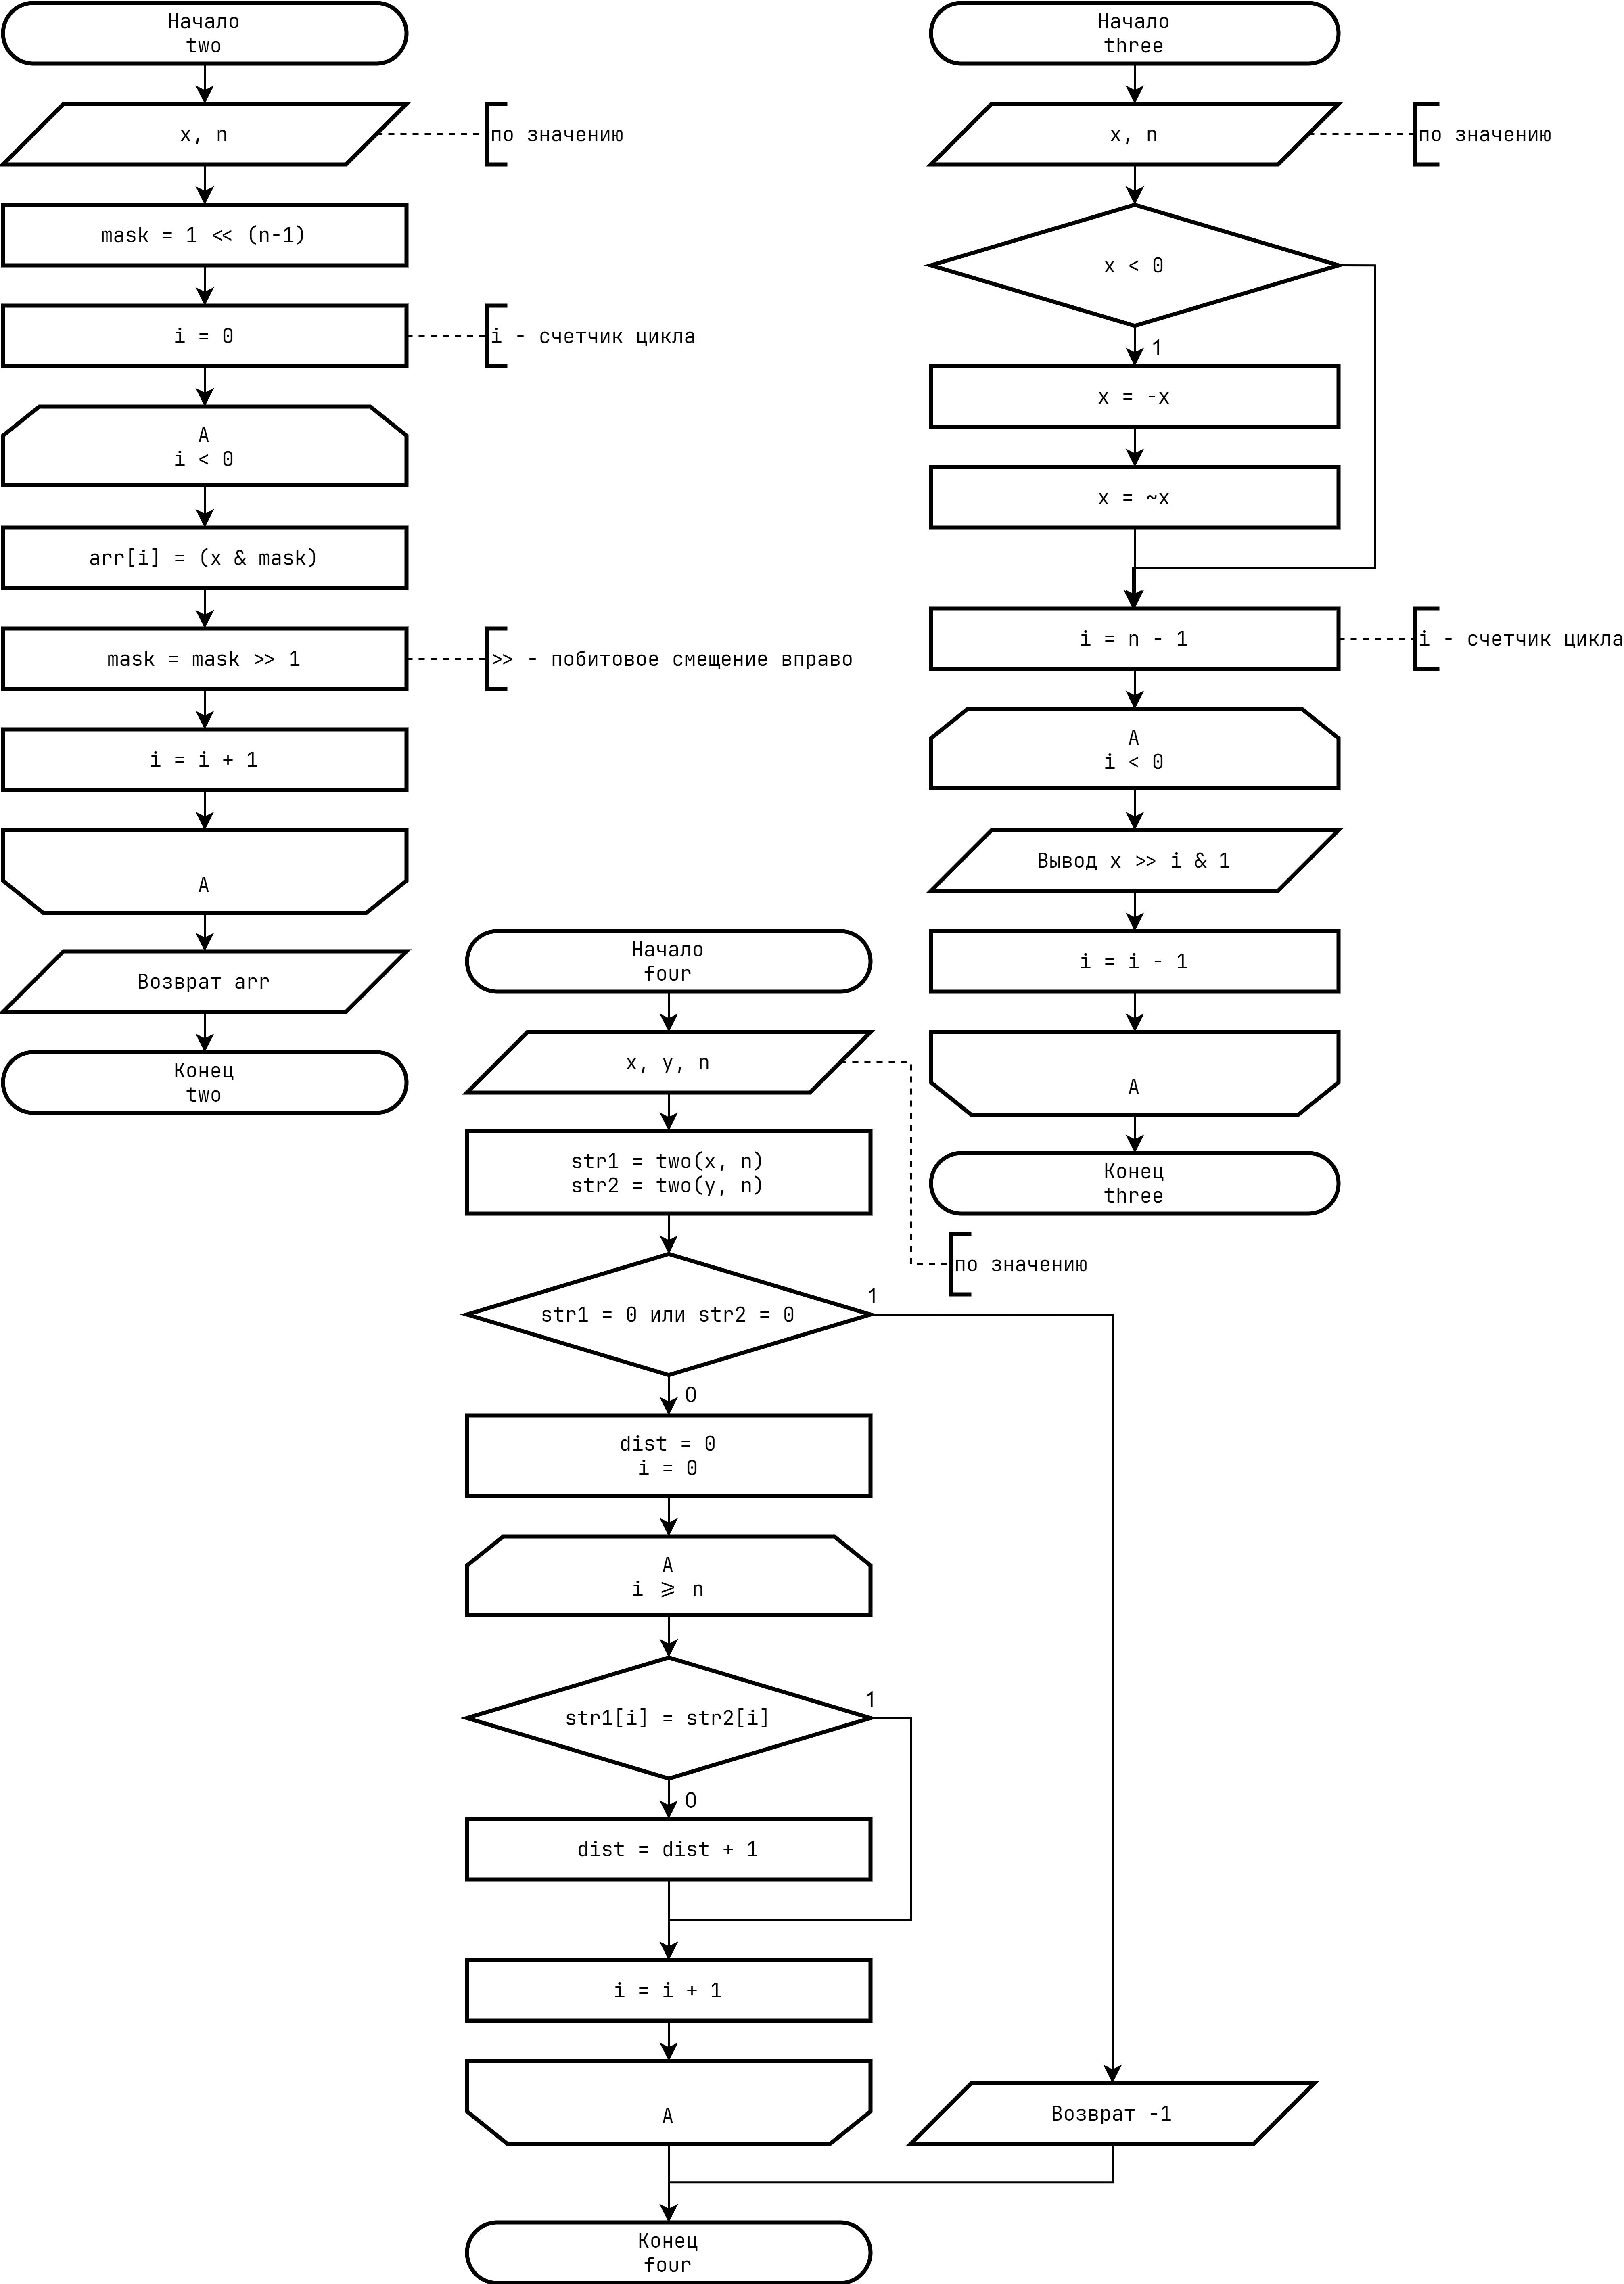
\includegraphics[height=0.9\textheight]{pics/flowchart_p2.png} 
	\caption*{Рисунок 1.2 - Схема алгоритма программы.}
\end{figure}.\\

\section*{Вывод}
В ходе работы удалось достичь цели --- закрепить знания о представлении чисел.
Были разработаны и проверены программы, которые работают правильно. Работа
помогла лучше понять тему и улучшить навыки программирования.

\section*{Приложеие А1}
\VerbatimInput[fontsize=\small]{code/main.c}

\end{document}